\section{Benchmark}
\label{eval}
The benchmarks analyses the performance and scalability (handling
concurrent requests) aspects of Yarn, WEBrick, Thin and Unicorn. It does not
include topics like security and reliability, which are important for
webservers, but out of scope for this project.

To evaluate Yarn, its performance will be analyzed first by itself, then it
is compared to the other Ruby webservers covered in Section~\ref{webservers}.
The measure of performance is how many requests the webserver can handle per
second. The tests were run on a 64-bit Linux machine with four cores and 8GB
RAM using Ruby (YARV) 1.9.3-rc1. The benchmarks were performed using Apache
Bench, which is a tool made to measure the number of requests per second a
webserver can perform.

\subsection{Yarn Performance}
To get an idea of the performance of Yarn, it was measured how many requests
per second (req/sec) it could handle at different counts of worker processes.
Figure~\ref{optwork} plots Yarn performance.

\begin{figure}[htb]
  \centering
  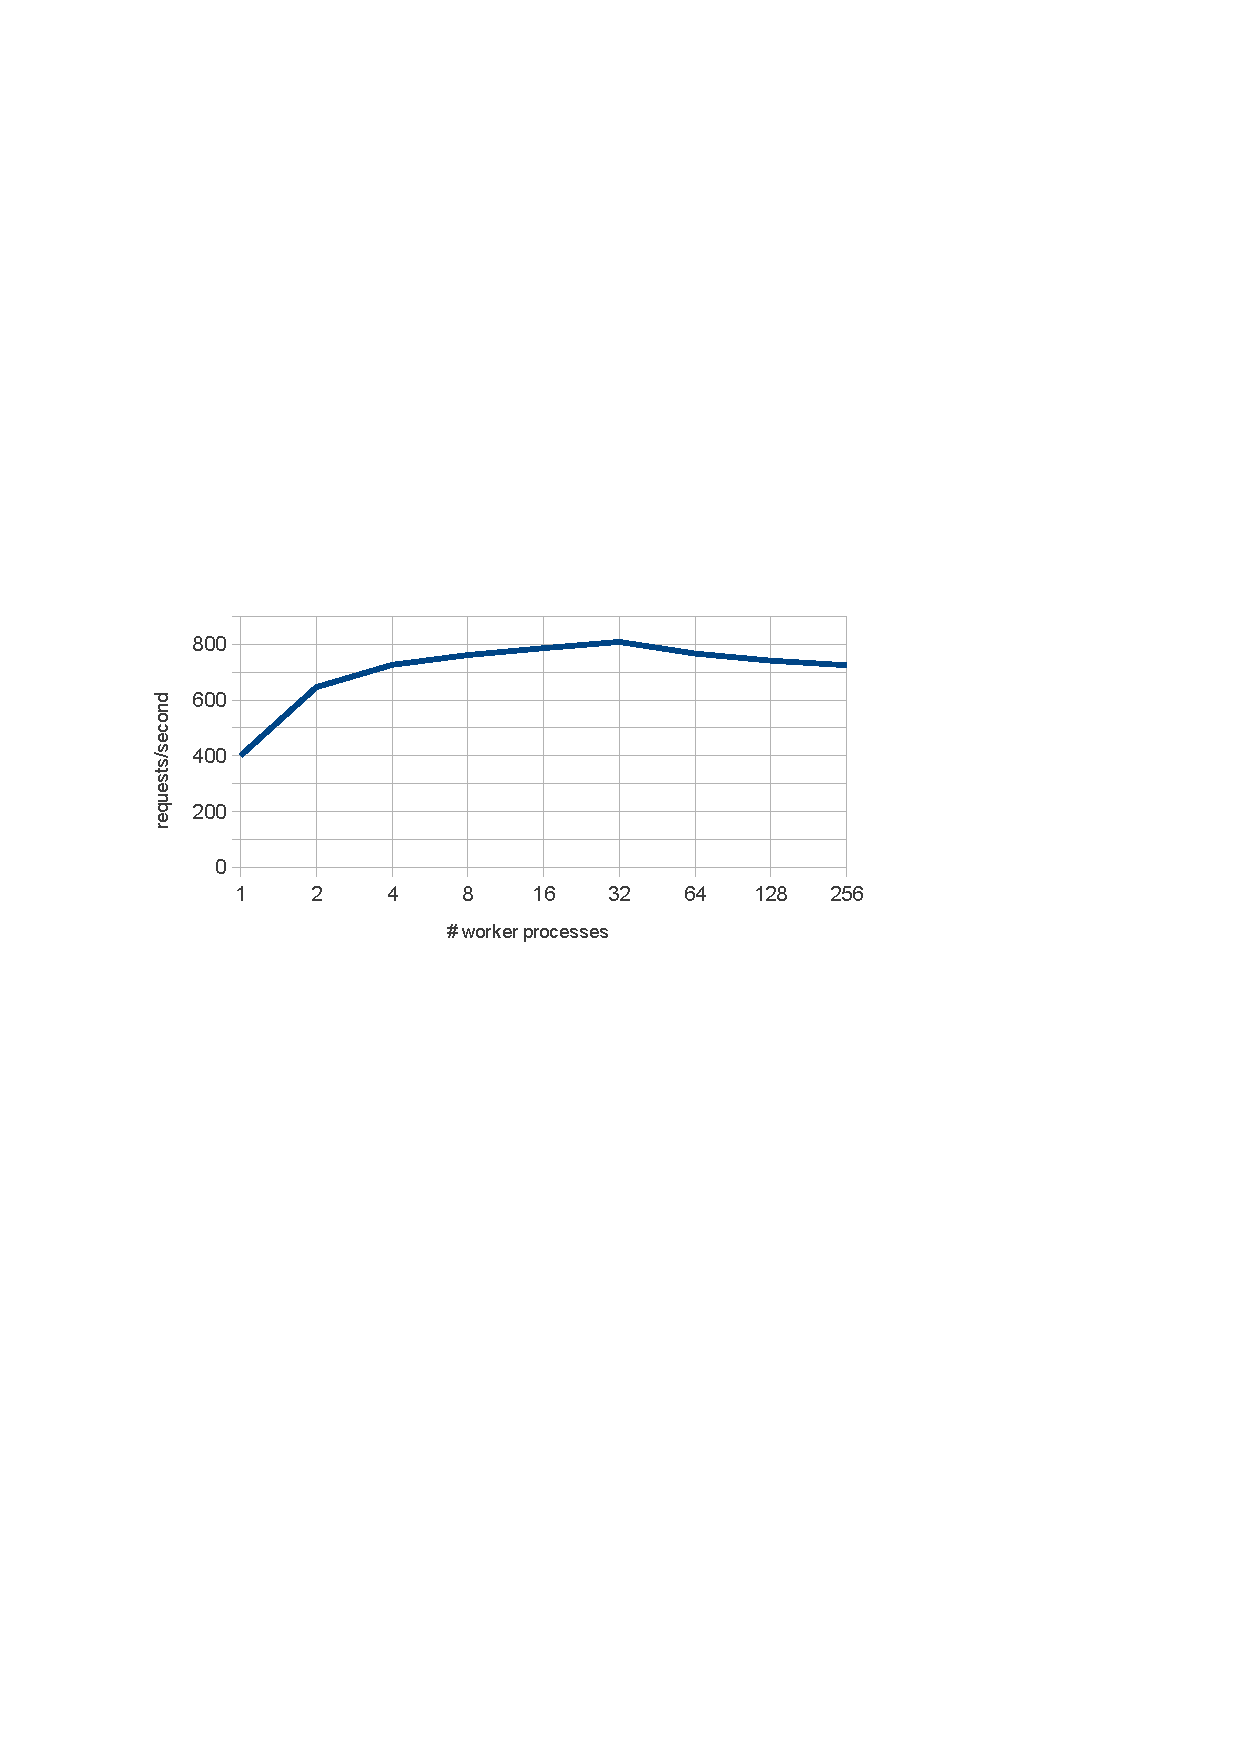
\includegraphics[width=0.99\textwidth]{benchmark/optimal_workers_crop.pdf}
  \caption{Yarn performance.}
  \label{optwork}
\end{figure}

Test runs above 256 processes bogged the computer down and were not included.
The cause of this was that context-switching and memory usage exceeded the
capabilities of the system. The best result was achieved with 32 worker
processes which maxed at 808 req/sec, and on average Yarn performed 706 req/sec. The
test consisted of making 2000 requests, 200 at a time, to Yarn serving a
simple Rack application (source/test\_objects/config.ru).

\subsection{Yarn Vs. Other Ruby Webservers}
The following benchmarks compare Yarn's performance compared to
other Ruby webservers. Listing~\ref{staticbench} shows the results of
measuring the webservers performance serving a simple static Rack application.
The test was performed doing 2000 requests, 20 at a time. The average of four
test runs was used to minimize outside factors from polluting the results.

\begin{figure}[htb]
  \centering
  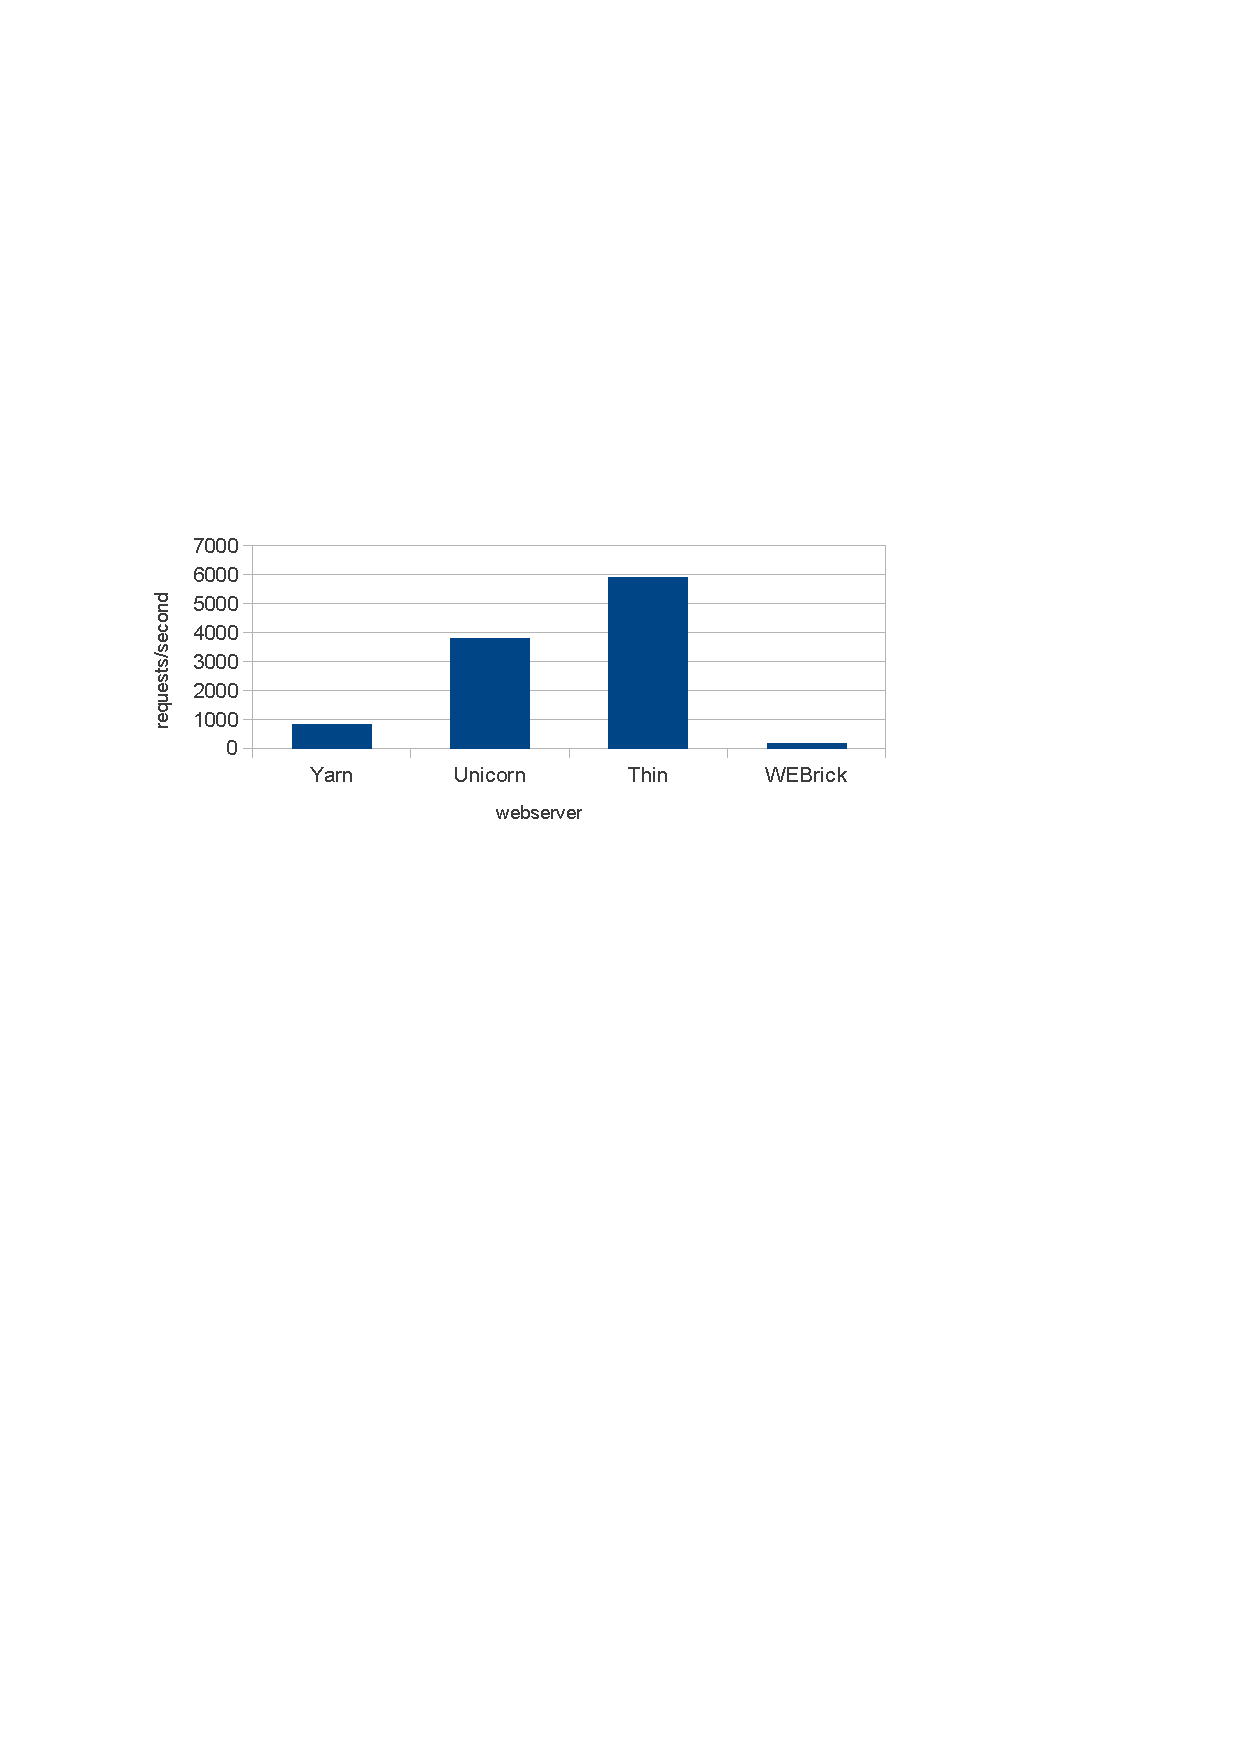
\includegraphics[width=1.0\textwidth]{benchmark/static.pdf}
  \caption{Serving a static Rack application.}
  \label{staticbench}
\end{figure}

Benchmarking with a static Rack application revealed that this was something
that Thin managed really well with 5915 req/sec on average.  Unicorn came
second with 3792 req/sec, Yarn third with around 820 req/sec and
WEBrick last with 180 req/sec. 

Thin's excellent performance is interpreted to be the result of not having to
do any context-switching as all requests are handled in one thread.
Furthermore, the impact of Thin and Unicorn's fast C HTTP parser has a
higher impact when the time spent parsing the request relatively high compared
to the amount of time spent creating the response. The bottleneck in Yarn's
implementation is currently the parser which performs a lot of string
computations. Had more time been available it would have been interesting to
see how it fared using the C parser from Unicorn.

% next BM
The results were quite different when a CPU intensive Rack application was
used. Listing~\ref{cpubench} shows the results of benchmarking with a Rack
application that calculates the Fibonacci sequence up to 10,000.

\begin{figure}[htb]
  \centering
  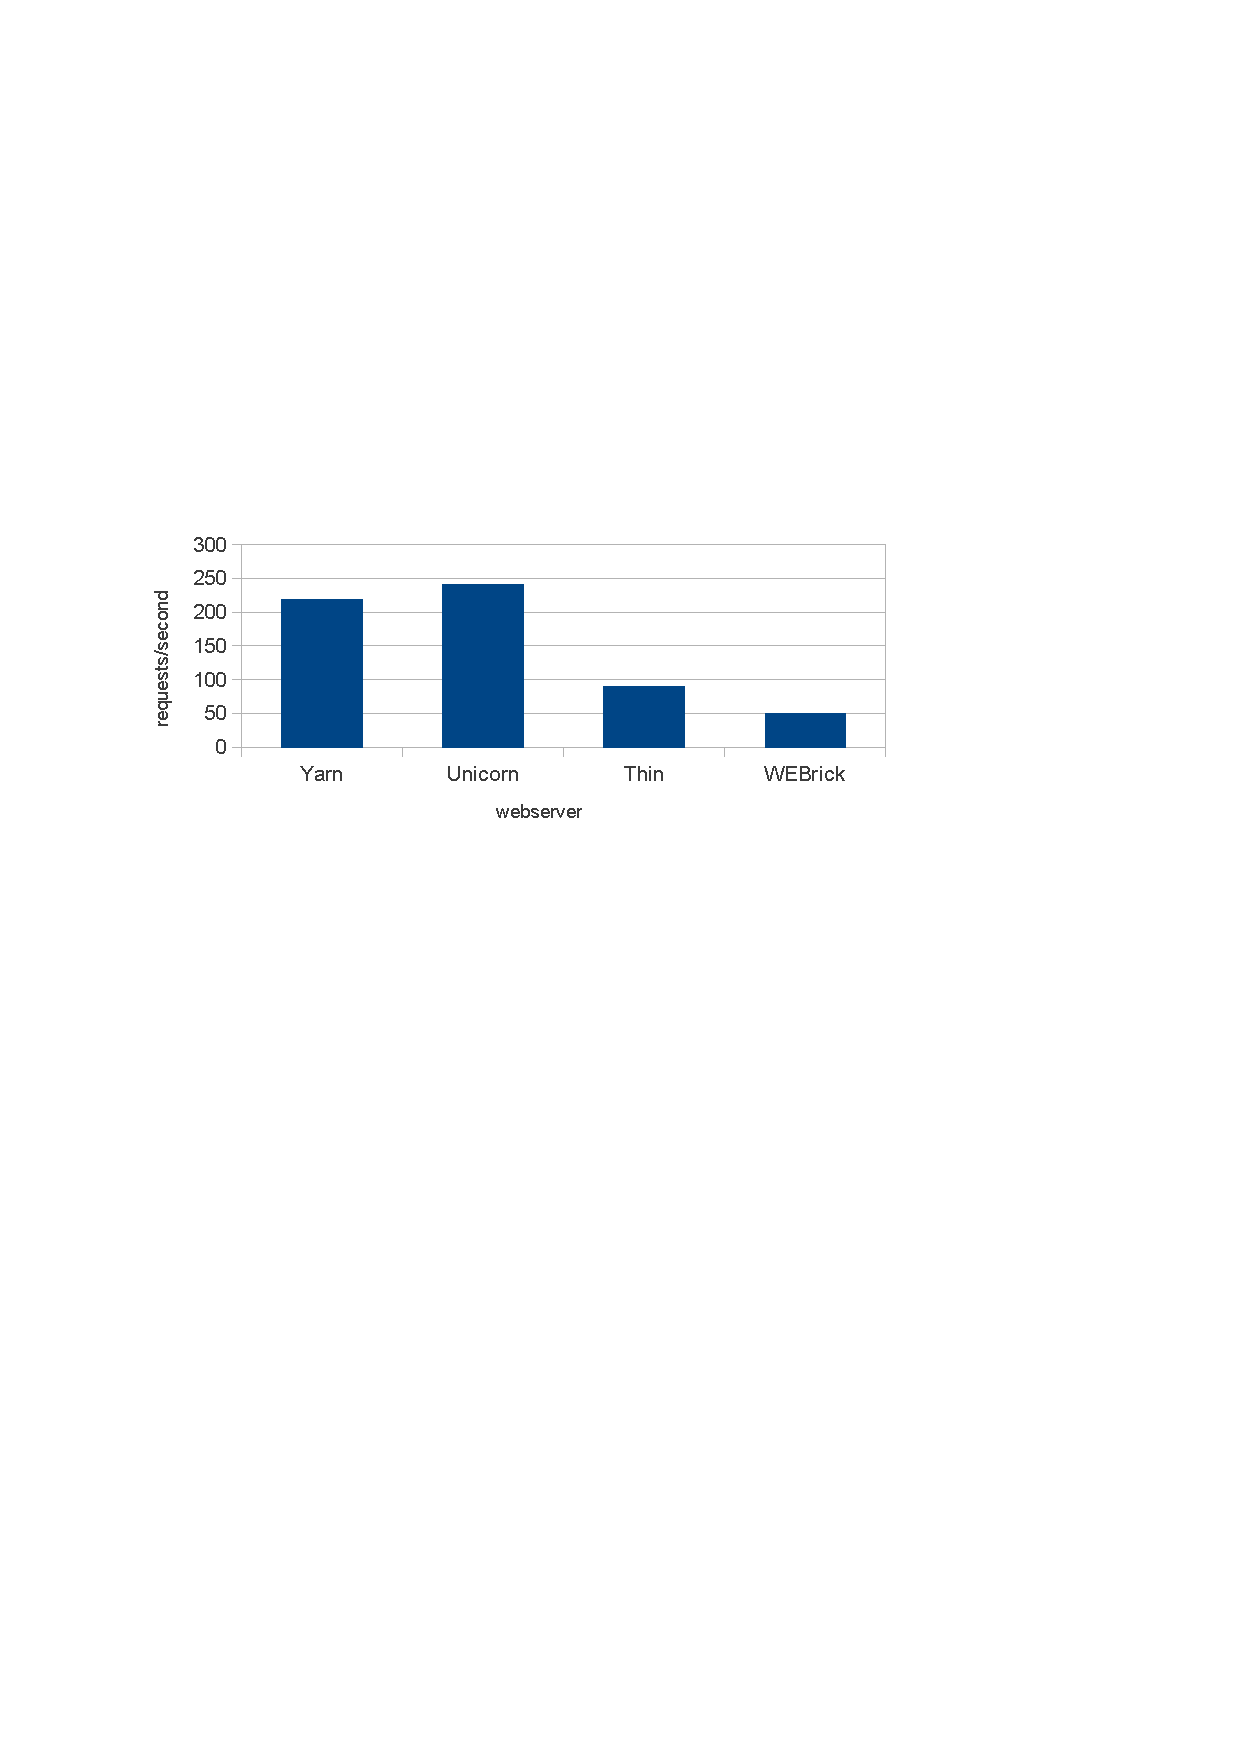
\includegraphics[width=1.0\textwidth]{benchmark/cpu.pdf}
  \caption{Serving a CPU intensive Rack application}
  \label{cpubench}
\end{figure}

With each request now having to run a CPU intensive computation, Unicorn came in
first with 240 req/sec, Yarn second with 218 req/sec, then Thin with 90
req/sec and lastly WEBrick with 50 req/sec. With a CPU intensive application,
the benefits of parallel processing is apparent, as is the case with
Unicorn and Yarn. Thin and WEBrick would probably perform similarly if
multiple instances and a load balancer was used.
